\documentclass[border=10pt]{standalone}
\usepackage{amsmath,amssymb}
\usepackage{tikz}
\usetikzlibrary{arrows.meta,calc,decorations.pathreplacing,patterns,shapes.geometric,positioning,shadings,plotmarks}

\begin{document}
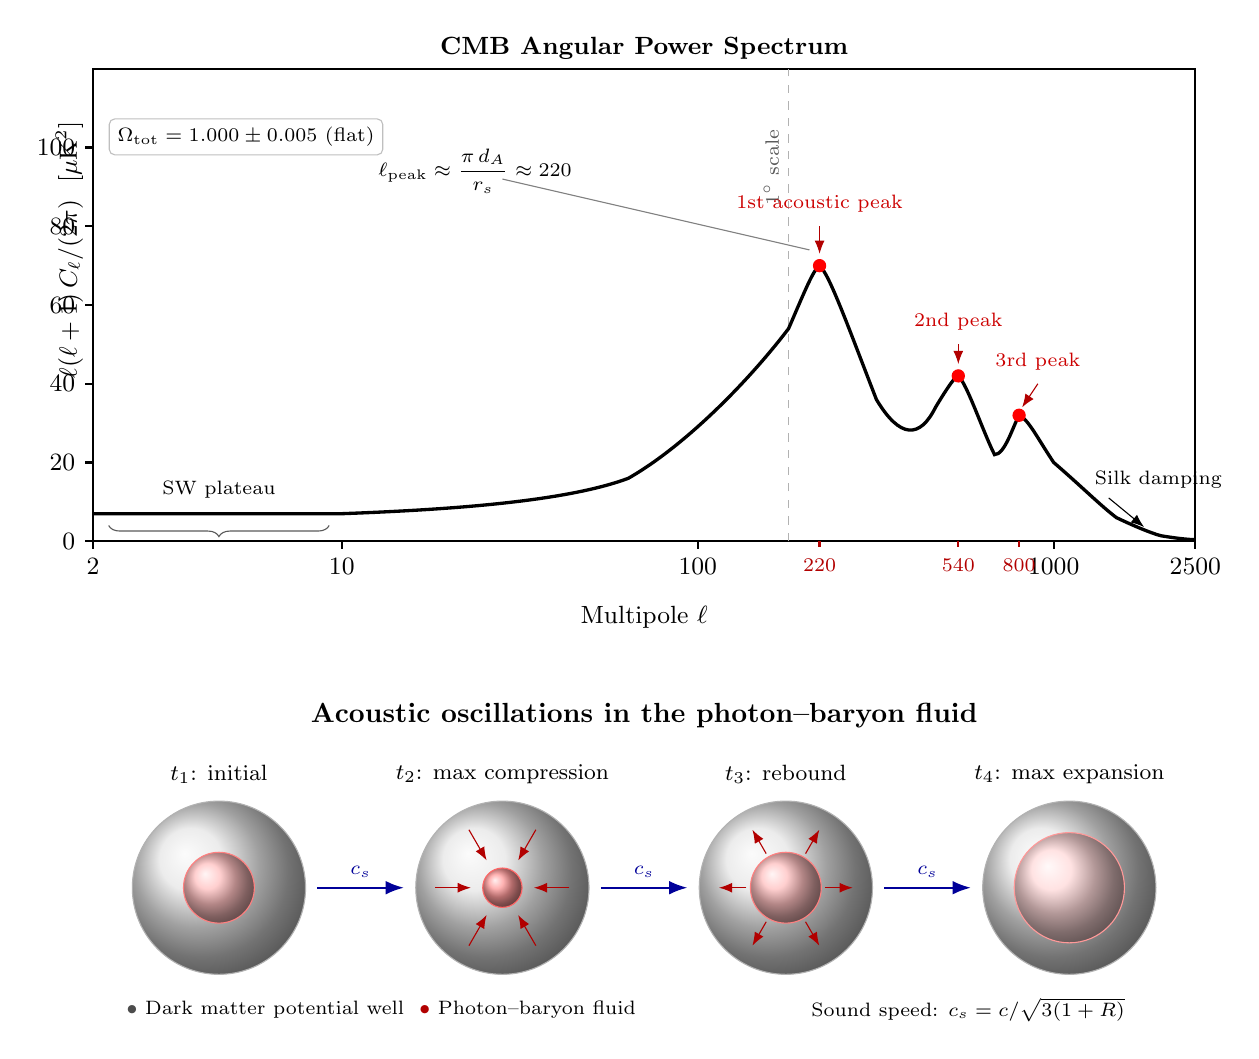
\begin{tikzpicture}[>=Latex, font=\small]

% ===================================================================
% TOP PANEL: CMB Angular Power Spectrum C_ell vs ell (log-x)
% ===================================================================

% --- Axes frame (top panel) ---
% Plot area: x in [0, 14] represents log10(ell) from log10(2) to log10(2500)
% We use a direct mapping: for a given ell, x = 14 * (log10(ell) - log10(2)) / (log10(2500) - log10(2))
% Simpler: we'll compute positions manually for key ells.
% y in [0, 6] represents amplitude in mu K^2 units (scaled so peak 1 at y=5)

\begin{scope}[shift={(0,0)}]
  % Axes
  \draw[thick] (0,0) -- (14,0) -- (14,6) -- (0,6) -- cycle;

  % --- X-axis tick positions (log scale) ---
  % Helper: x(ell) = 14*(log10(ell) - log10(2))/(log10(2500) - log10(2))
  % log10(2500/2) = log10(1250) ~ 3.0969
  % x(ell) = 14 * (log10(ell) - 0.3010) / 3.0969
  % Ticks at: 2, 10, 100, 220, 540, 800, 1000, 2000, 2500
  % x(2)     = 0
  % x(10)    = 14*(1.0 - 0.3010)/3.0969     = 3.160
  % x(100)   = 14*(2.0 - 0.3010)/3.0969     = 7.681
  % x(180)   = 14*(2.2553 - 0.3010)/3.0969  = 8.834
  % x(220)   = 14*(2.3424 - 0.3010)/3.0969  = 9.228
  % x(540)   = 14*(2.7324 - 0.3010)/3.0969  = 10.990
  % x(800)   = 14*(2.9031 - 0.3010)/3.0969  = 11.762
  % x(1000)  = 14*(3.0 - 0.3010)/3.0969     = 12.202
  % x(1500)  = 14*(3.1761 - 0.3010)/3.0969  = 12.998
  % x(2000)  = 14*(3.3010 - 0.3010)/3.0969  = 13.563
  % x(2500)  = 14

  % Major ticks on x-axis
  \foreach \x/\lab in {0/2, 3.160/10, 7.681/100, 12.202/1000, 14/2500}{
    \draw[thick] (\x,0) -- (\x,-0.1);
    \node[below] at (\x,-0.1) {$\lab$};
  }
  % Extra minor ticks (labeled peaks)
  \foreach \x/\lab in {9.228/220, 10.990/540, 11.762/800}{
    \draw[red!70!black, thick] (\x,0) -- (\x,-0.07);
    \node[red!70!black, below, font=\scriptsize] at (\x,-0.1) {$\lab$};
  }

  % Y-axis ticks (amplitude in mu K^2)
  \foreach \y/\lab in {0/0, 1/20, 2/40, 3/60, 4/80, 5/100}{
    \draw[thick] (0,\y) -- (-0.1,\y);
    \node[left] at (-0.1,\y) {$\lab$};
  }

  % Axis labels
  \node[below=0.6cm] at (7,-0.1) {Multipole $\ell$};
  \node[rotate=90, above=0.7cm] at (0,3) {$\ell(\ell+1)\,C_\ell/(2\pi)\ \ [\mu\mathrm{K}^2]$};
  \node[above] at (7,6) {\textbf{CMB Angular Power Spectrum}};

  % --- 1 degree reference line at ell = 180 ---
  \draw[gray!60, dashed, thin] (8.834,0) -- (8.834,6);
  \node[gray!70!black, above, font=\scriptsize, rotate=90] at (8.834,4.7) {\ $1^\circ$ scale};

  % --- Main curve: Sachs-Wolfe plateau + three peaks + Silk damping ---
  % Construct via smooth path through control points (ell, amplitude)
  % All coords in (x_of_ell, y_value/20)
  % Plateau region (ell 2 -> 30): low, around 7 muK^2 (y = 0.35)
  % Rise to first peak (ell 220): amplitude 70 muK^2 -> y = 3.5
  % Trough between peaks 1 and 2 (~ell 420): ~25 -> y = 1.25
  % Second peak (ell 540): ~42 -> y = 2.1
  % Trough (~ell 680): ~20 -> y = 1.0
  % Third peak (ell 800): ~32 -> y = 1.6
  % Silk damping tail: drops rapidly to ell 2500

  % Draw main curve as a smooth path
  \draw[black, very thick]
    (0, 0.35)                                    % ell=2,    plateau ~7 uK^2
    .. controls (1.5, 0.35) and (2.5, 0.35) ..
    (3.160, 0.35)                                % ell=10
    .. controls (4.5, 0.40) and (6.0, 0.50) ..
    (6.8, 0.80)                                  % ell=50 ish, rising
    .. controls (7.5, 1.2) and (8.3, 2.0) ..
    (8.834, 2.7)                                 % ell=180, rising steeply
    .. controls (9.05, 3.20) and (9.15, 3.45) ..
    (9.228, 3.50)                                % ell=220 FIRST PEAK (70 uK^2)
    .. controls (9.35, 3.40) and (9.6, 2.70) ..
    (9.95, 1.80)                                 % trough after peak 1
    .. controls (10.25, 1.30) and (10.50, 1.30) ..
    (10.70, 1.70)                                % rising to peak 2
    .. controls (10.88, 2.00) and (10.96, 2.10) ..
    (10.990, 2.10)                               % ell=540 SECOND PEAK (~42)
    .. controls (11.10, 2.00) and (11.30, 1.40) ..
    (11.45, 1.10)                                % trough after peak 2
    .. controls (11.58, 1.10) and (11.68, 1.45) ..
    (11.762, 1.60)                               % ell=800 THIRD PEAK (~32)
    .. controls (11.88, 1.55) and (12.00, 1.30) ..
    (12.202, 1.00)                               % ell=1000
    .. controls (12.55, 0.70) and (12.80, 0.45) ..
    (12.998, 0.30)                               % ell=1500, Silk damping begins
    .. controls (13.25, 0.18) and (13.45, 0.10) ..
    (13.563, 0.07)                               % ell=2000
    .. controls (13.80, 0.03) and (13.95, 0.02) ..
    (14, 0.02);                                  % ell=2500

  % --- Peak markers ---
  \filldraw[red] (9.228, 3.50) circle (2.2pt);
  \filldraw[red] (10.990, 2.10) circle (2.2pt);
  \filldraw[red] (11.762, 1.60) circle (2.2pt);

  % Peak labels with arrows
  \node[red!80!black, font=\scriptsize, anchor=south] at (9.228, 4.05) {1st acoustic peak};
  \draw[red!70!black, ->, thin] (9.228, 4.0) -- (9.228, 3.65);

  \node[red!80!black, font=\scriptsize, anchor=south] at (10.990, 2.55) {2nd peak};
  \draw[red!70!black, ->, thin] (10.990, 2.50) -- (10.990, 2.25);

  \node[red!80!black, font=\scriptsize, anchor=south] at (12.00, 2.05) {3rd peak};
  \draw[red!70!black, ->, thin] (12.00, 2.00) -- (11.80, 1.70);

  % --- SW plateau label ---
  \draw[decorate, decoration={brace, amplitude=4pt, mirror}, gray!70!black, thin]
    (0.2, 0.20) -- (3.000, 0.20);
  \node[gray!30!black, font=\scriptsize, anchor=north] at (1.6, 0.0) {};
  \node[font=\scriptsize, anchor=south] at (1.6, 0.42) {SW plateau};

  % --- Silk damping label ---
  \node[font=\scriptsize, anchor=south west] at (12.6, 0.55) {Silk damping};
  \draw[thin, ->] (12.90, 0.55) -- (13.35, 0.18);

  % Formula for first peak
  \node[black, font=\scriptsize, anchor=west] at (3.5, 4.7)
    {$\ell_{\mathrm{peak}} \approx \dfrac{\pi\, d_A}{r_s} \approx 220$};
  \draw[thin, gray] (5.2, 4.6) -- (9.1, 3.7);

  % Flatness box (bottom left)
  \node[font=\scriptsize, anchor=south west, draw=gray!50, rounded corners=2pt,
        fill=white, inner sep=3pt] at (0.2, 4.9)
    {$\Omega_{\mathrm{tot}} = 1.000 \pm 0.005$ (flat)};

\end{scope}

% ===================================================================
% BOTTOM PANEL: Acoustic oscillation cartoon - four snapshots
% ===================================================================

\begin{scope}[shift={(0,-4.4)}]
  \node[font=\bfseries, anchor=south] at (7, 1.9)
    {Acoustic oscillations in the photon--baryon fluid};

  % Four time snapshots centered horizontally: t1 at x=1.6, t2 at x=5.2, t3 at x=8.8, t4 at x=12.4
  \foreach \cx/\tlab/\phase in {1.6/$t_1$/initial/2.4/, 5.2/$t_2$/compression/, 8.8/$t_3$/rebound/, 12.4/$t_4$/expansion/}{
  }

  % --- Snapshot t1: Initial perturbation ---
  % Dark matter halo (gray cloud)
  \shade[ball color=gray!20] (1.6, 0) circle (1.1cm);
  \draw[gray!60, thin] (1.6, 0) circle (1.1cm);
  % Photon-baryon fluid (pink ball, medium)
  \shade[ball color=red!25] (1.6, 0) circle (0.45cm);
  \draw[red!50, thin] (1.6, 0) circle (0.45cm);
  \node[font=\footnotesize, anchor=south] at (1.6, 1.2) {$t_1$: initial};

  % --- Snapshot t2: Maximum compression ---
  \shade[ball color=gray!20] (5.2, 0) circle (1.1cm);
  \draw[gray!60, thin] (5.2, 0) circle (1.1cm);
  \shade[ball color=red!40] (5.2, 0) circle (0.25cm);
  \draw[red!60, thin] (5.2, 0) circle (0.25cm);
  % inward pressure arrows
  \foreach \a in {0, 60, 120, 180, 240, 300}{
    \draw[red!70!black, ->, thin] ([shift={(\a:0.85cm)}]5.2, 0) -- ([shift={(\a:0.4cm)}]5.2, 0);
  }
  \node[font=\footnotesize, anchor=south] at (5.2, 1.2) {$t_2$: max compression};

  % --- Snapshot t3: Rebound ---
  \shade[ball color=gray!20] (8.8, 0) circle (1.1cm);
  \draw[gray!60, thin] (8.8, 0) circle (1.1cm);
  \shade[ball color=red!25] (8.8, 0) circle (0.45cm);
  \draw[red!50, thin] (8.8, 0) circle (0.45cm);
  % outward arrows
  \foreach \a in {0, 60, 120, 180, 240, 300}{
    \draw[red!70!black, ->, thin] ([shift={(\a:0.5cm)}]8.8, 0) -- ([shift={(\a:0.85cm)}]8.8, 0);
  }
  \node[font=\footnotesize, anchor=south] at (8.8, 1.2) {$t_3$: rebound};

  % --- Snapshot t4: Maximum expansion ---
  \shade[ball color=gray!20] (12.4, 0) circle (1.1cm);
  \draw[gray!60, thin] (12.4, 0) circle (1.1cm);
  \shade[ball color=red!15] (12.4, 0) circle (0.70cm);
  \draw[red!40, thin] (12.4, 0) circle (0.70cm);
  \node[font=\footnotesize, anchor=south] at (12.4, 1.2) {$t_4$: max expansion};

  % --- Connecting arrows between snapshots ---
  \draw[->, thick, blue!60!black] (2.85, 0) -- (3.95, 0) node[midway, above, font=\scriptsize] {$c_s$};
  \draw[->, thick, blue!60!black] (6.45, 0) -- (7.55, 0) node[midway, above, font=\scriptsize] {$c_s$};
  \draw[->, thick, blue!60!black] (10.05, 0) -- (11.15, 0) node[midway, above, font=\scriptsize] {$c_s$};

  % --- Legend ---
  \node[font=\scriptsize, anchor=west] at (0.3, -1.55)
    {\textcolor{gray!60!black}{$\bullet$} Dark matter potential well
     \ \textcolor{red!70!black}{$\bullet$} Photon--baryon fluid};
  \node[font=\scriptsize, anchor=west] at (9.0, -1.55)
    {Sound speed: $c_s = c/\sqrt{3(1+R)}$};
\end{scope}

\end{tikzpicture}
\end{document}
